\documentclass[12pt]{article}
\usepackage[utf8]{inputenc}
\usepackage{float}
\usepackage{amsmath}

\usepackage[hmargin=3cm,vmargin=6.0cm]{geometry}
%\topmargin=0cm
\topmargin=-2cm
\addtolength{\textheight}{6.5cm}
\addtolength{\textwidth}{2.0cm}
%\setlength{\leftmargin}{-5cm}
\setlength{\oddsidemargin}{0.0cm}
\setlength{\evensidemargin}{0.0cm}

%misc libraries goes here
\usepackage{amsthm}
\usepackage{mathtools}
\usepackage{listings}
\usepackage{xcolor}
\usepackage{graphicx}
\usepackage[T1]{fontenc}

\definecolor{codegreen}{rgb}{0,0.6,0}
\definecolor{codegray}{rgb}{0.5,0.5,0.5}
\definecolor{codepurple}{rgb}{0.58,0,0.82}
\definecolor{backcolour}{rgb}{0.95,0.95,0.92}

\lstdefinestyle{mystyle}{
    backgroundcolor=\color{backcolour},
    commentstyle=\color{codegreen},
    keywordstyle=\color{magenta},
    numberstyle=\tiny\color{codegray},
    stringstyle=\color{codepurple},
    basicstyle=\ttfamily\footnotesize,
    breakatwhitespace=false,
    breaklines=true,
    captionpos=b,
    keepspaces=true,
    numbers=none,
    numbersep=5pt,
    showspaces=false,
    showstringspaces=false,
    showtabs=false,
    tabsize=2
}

\lstset{style=myStyle}

\begin{document}

\section*{Student Information } 
%Write your full name and id number between the colon and newline
%Put one empty space character after colon and before newline
Full Name : Murat Bolu \\
Id Number : 2521300 \\

% Write your answers below the section tags
\section*{Answer 1}

\subsection*{a)} 

The expected value $E(X)$ for random variables with finitely many outcomes is
equal to $\displaystyle\sum_{x}^{}xP(x)$.
Therefore, assuming all dice are fair, i.e. all sides have the same probability
of occurring,

\begin{gather*}
    E(\text{Blue die}) = 1 \cdot \tfrac{1}{6}
                       + 2 \cdot \tfrac{1}{6}
                       + 3 \cdot \tfrac{1}{6}
                       + 4 \cdot \tfrac{1}{6}
                       + 5 \cdot \tfrac{1}{6}
                       + 6 \cdot \tfrac{1}{6} = 3.5 \\
    \\
    E(\text{Yellow die}) = 1 \cdot \tfrac{1}{8}
                         + 1 \cdot \tfrac{1}{8}
                         + 1 \cdot \tfrac{1}{8}
                         + 3 \cdot \tfrac{1}{8}
                         + 3 \cdot \tfrac{1}{8}
                         + 3 \cdot \tfrac{1}{8}
                         + 4 \cdot \tfrac{1}{8}
                         + 8 \cdot \tfrac{1}{8} = 3 \\
    \\
    E(\text{Red die}) = 2 \cdot \tfrac{1}{10}
                      + 2 \cdot \tfrac{1}{10}
                      + 2 \cdot \tfrac{1}{10}
                      + 2 \cdot \tfrac{1}{10}
                      + 2 \cdot \tfrac{1}{10}
                      + 3 \cdot \tfrac{1}{10}
                      + 3 \cdot \tfrac{1}{10}
                      + 4 \cdot \tfrac{1}{10}
                      + 4 \cdot \tfrac{1}{10}
                      + 6 \cdot \tfrac{1}{10} = 3
\end{gather*}

\subsection*{b)} 

I would roll the blue die thrice. By using the linearity of expectation,

\begin{align*}
    \shortintertext{
        \[ E(\text{3 Blue dice}) [0.5ex]= 3 \cdot E(\text{Blue die}) = 10.5 \]
    } 
    E(\text{One of each dice}) &= E(\text{Blue die})
                                + E(\text{Yellow die})
                                + E(\text{Red die}) \\
                               &= 3.5 + 3 + 3 \\
                               &= 9.5
    \shortintertext{\[ 10.5 > 9.5 \]}
\end{align*}

\vspace{-15mm}
\subsection*{c)} 

If the value of the yellow die is 8, then it is no longer a random variable.
Its expected value is trivially 8.
I would choose rolling one of each die this time, since,

\begin{align*}
    E(\text{One of each dice}) &= E(\text{Blue die})
                                + E(\text{Yellow die})
                                + E(\text{Red die}) \\
                               &= 3.5 + 8 + 3 \\
                               &= 14.5
    \shortintertext{\[ 14.5 > 10.5 \]}
\end{align*}

\subsection*{d)} 

By using Bayes theorem and the law of total probability,

\begin{align*}
    P(\text{Die is red} \mid \text{Value is 3})
        &= \frac{P(\text{Value is 3} \mid \text{Die is red})
                    \cdot P(\text{Die is red})}
                {P(\text{Value is 3})} \\[1.5ex]
        &= \frac{P(\text{V}_3 \mid \text{D}_\text{r})
                    \cdot P(\text{D}_\text{r})}
                {P(\text{V}_3 \mid \text{D}_\text{b})
                    \cdot P(\text{D}_\text{b}) +
                 P(\text{V}_3 \mid \text{D}_\text{y})
                    \cdot P(\text{D}_\text{y}) +
                 P(\text{V}_3 \mid \text{D}_\text{r})
                    \cdot P(\text{D}_\text{r})} \\[1.5ex]
        &= \frac{\tfrac{2}{10} \cdot \tfrac{1}{3}}
                {\tfrac{1}{6} \cdot \tfrac{1}{3}
                + \tfrac{3}{8} \cdot \tfrac{1}{3}
                + \tfrac{2}{10} \cdot \tfrac{1}{3}} \\[1.5ex]
        &= \frac{\tfrac{2}{10}}
                {\tfrac{1}{6} + \tfrac{3}{8} + \tfrac{2}{10}} \\[1.5ex]
        &= \frac{\tfrac{1}{5}}
                {\tfrac{1}{6} + \tfrac{3}{8} + \tfrac{1}{5}} \\[1.5ex]
        &= \frac{24}{20 + 45 + 24} \\[1.5ex]
        &= \frac{24}{89}
\end{align*}

\subsection*{e)} 

The total value can be 5 in four different ways, namely $(1, 4), (2, 3), (3, 2),
(4, 1)$, where the first element represent the value of the blue die and the
second element represent the value of the yellow die.
Since these are independent events, simple multiplication is sufficient.

\begin{align*}
    P(\text{Blue die is 1}) \cdot P(\text{Yellow die is 4})
        &= \tfrac{1}{6} \cdot \tfrac{1}{8} = \tfrac{1}{48} \\[0.5ex]
    P(\text{Blue die is 2}) \cdot P(\text{Yellow die is 3})
        &= \tfrac{1}{6} \cdot \tfrac{3}{8} = \tfrac{3}{48} \\[0.5ex]
    P(\text{Blue die is 3}) \cdot P(\text{Yellow die is 2})
        &= \tfrac{1}{6} \cdot \tfrac{0}{8} = 0 \\[0.5ex]
    P(\text{Blue die is 4}) \cdot P(\text{Yellow die is 1})
        &= \tfrac{1}{6} \cdot \tfrac{3}{8} = \tfrac{3}{48} \\[0.5ex]
    \frac{1}{48} + \frac{3}{48} + 0 + \frac{3}{48} = \frac{7}{48}
\end{align*}

\newpage

\section*{Answer 2}

\subsection*{a)} 

The event of a specific distributor offering a discount that day can be thought
of being a Bernouilli trial, and the probability of a specific amount of
distributors offering a discount that day can be calculated using Binomial
distribution.
Since Company A has a large amount of distributors and a small chance of
offering a discount, we can use Poisson approximation of Binomial distribution
to calculate the probability of at least four distributors offering a discount
tomorrow.
\newline
The number of distributors are $n = 80$, chance of offering a discount is
$p = 0.025$, and the expected value of discounts per day are $n \cdot p = 2$.
The probability of at least four distributors offering a discount tomorrow is
one minus the cumulative probability of at most three distributors offering a
discount, i.e. $1 - F_Y(3) = 0.1429$ , where $F_Y$ is the cumulative
distribution function of Poisson distribution with $\lambda = 2$.

\subsection*{b)} 

Assuming the customer is only going to buy a phone when there is a discount
in $A$ or $B$, one can calculate the probability of buying a phone by
subtracting the probability of no discounts happening in two days from 1.
\newline
There will be no discounts if both $A$ and $B$ have no discounts.
\begin{itemize}
    \item $A$ will have no discounts with the probability $P(0) = 0.0183$,
    where $P$ is the probability density function of Poisson distribution with
    $\lambda = 4$, since we are looking at a two day timespan.
    \item $B$ will have no discounts with the probability
    $0.9 \cdot 0.9 = 0.81$.
    \item They will both have no discounts with the probability
    $0.0183 \cdot 0.81 = 0.0148$.
\end{itemize}
Therefore, the customer will be able to buy the phone in two days with the
probability $1 - 0.0148 = 0.9852$.

\newpage

\section*{Answer 3}

The Octave code is as follows,
\begin{lstlisting}[language=Octave]
    N = 1000;

    % F is the first iteration where we roll one die of each color
    F = rand(3, N);
    F = F.*[6; 8; 10];
    F = ceil(F);
    for i = 1:N
      F(:,i) = getValues(F(:,i));
    end
    F = sum(F);
    
    % S is the second iteration where we roll blue die thrice
    S = rand(3, N);
    S = S.*[6; 6; 6];
    S = ceil(S);
    S = sum(S);
    
    % isBigger is the 1 x N matrix with binary outcomes
    isBigger = (S > F);
    
    % Let F and S be the total average and isBigger the percentage
    % of times S was bigger than F
    F = sum(F)/N;
    S = sum(S)/N;
    isBigger = sum(isBigger)/length(isBigger)*100;
    
    printf("First option: %.2f\nSecond option: %.2f\
    \nPercentage of cases: %2.2f%%\n", F, S, isBigger)
    
    function out = getValues(x)
      b = x(1); y = x(2); r = x(3);
      b = [1 2 3 4 5 6](1, b);
      y = [1 1 1 3 3 3 4 8](1, y);
      r = [2 2 2 2 2 3 3 4 4 6](1, r);
      out = [b; y; r];
    endfunction
\end{lstlisting}

\newpage

\noindent
with a screenshot of some outputs,

\begin{center}
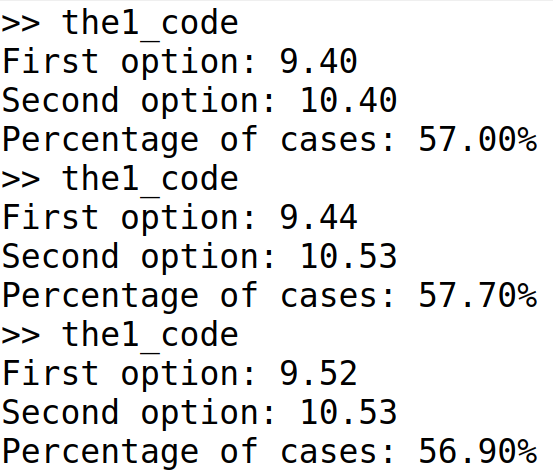
\includegraphics[scale = 0.5]{the1_outputs.png}
\end{center}

The findings agree with our calculations.
First option is close to $9.5$ and the second option is close to $10.5$.
The second option has a slight advantage compared to the first one, as we can
see in the percentage of cases it triumphed over the first one.
However, it is not a huge difference.

\end{document}